% -----------------------------------------------
% Template for ISMIR 2014
% (based on earlier ISMIR templates)
% -----------------------------------------------

\documentclass{article}
\usepackage{ismir2014,amsmath,cite}
\usepackage{graphicx}
\usepackage{brian}

% Title.
% ------
\title{Analyzing song structure with spectral clustering}

% Single address
% To use with only one author or several with the same address
% ---------------
%\oneauthor
% {Names should be omitted for double-blind reviewing}
% {Affiliations should be omitted for double-blind reviewing}

% Two addresses
% --------------
%\twoauthors
%  {First author} {School \\ Department}
%  {Second author} {Company \\ Address}

% Three addresses
% --------------
\threeauthors
  {First author} {Affiliation1 \\ {\tt author1@ismir.edu}}
  {Second author} {\bf Retain these fake authors in\\\bf submission to preserve the formatting}
  {Third author} {Affiliation3 \\ {\tt author3@ismir.edu}}

% Four addresses
% --------------
%\fourauthors
%  {First author} {Affiliation1 \\ {\tt author1@ismir.edu}}
%  {Second author}{Affiliation2 \\ {\tt author2@ismir.edu}}
%  {Third author} {Affiliation3 \\ {\tt author3@ismir.edu}}
%  {Fourth author} {Affiliation4 \\ {\tt author4@ismir.edu}}

\begin{document}
%
\maketitle
%
\begin{abstract}
Many approaches to analyzing the structure of a musical recording involve detecting
sequential patterns within a self-similarity matrix derived from time-series features.
Such patterns ideally capture repeated sequences, which then form the building blocks
of large-scale structure.

In this work, techniques from spectral graph theory are applied to analyze repeated
patterns in musical recordings.  The proposed method produces a low-dimensional
encoding of repetition structure, and exposes the hierarchical relationships among
structural components at differing levels of granularity.  Finally, we demonstrate how
to apply the proposed method to the task of music segmentation.
\end{abstract}
%
\section{Introduction}\label{sec:introduction}
Detecting repeated forms in audio is fundamental to the analysis of structure in many 
forms of music.  While small-scale repetitions --- such as each instance of an
individual chord --- are simple to detect, accurately combining multiple 
small-scale repetitions into larger structures is a challenging algorithmic task.
Much of the current research on this topic begins by calculating local, frame-wise
similarities over acoustic features (usually harmonic), and then searching for
patterns in the all-pairs self-similarity matrix~\cite{foote2000automatic}.

In the majority of existing work on structural segmentation, the analysis is
\emph{linear}, in the sense that the representation does not explicitly encode nesting
or hierarchical structure in the repeated forms.  Instead, novelty curves are commonly
used to detect when one section transitions into the
next~\cite{serra2012unsupervised}. 

% TODO:   2014-05-06 08:09:31 by Brian McFee <brm2132@columbia.edu>
%  why are we doing this work?
%   one level of segmentation is never enough
%   we want a full parse of the recording
%   how do nested structures relate to each-other?


\subsection{Our contributions}
In this paper, we formulate the structure analysis problem in the context of spectral
graph theory.  By combining local sequence information with long-term repeated forms,
and analyzing the eigenvectors of the resulting graph Laplacian, we produce a compact
representation that effectively encodes repetition structure at multiple levels of
granularity.  To effectively link repeating sequences, we formulate an optimally
weighted combination of local timbre consistency and long-term repetition descriptors.

To motivate the analysis technique, we demonstrate its use for the
standard task of flat structural annotation.  However, we emphasize that the approach
itself could have more general applications in analyzing hierarchical structure.

\subsection{Related work}

The structural repetition features used in this work are inspired by those of
Serr\`{a}~\etal~\cite{serra2012unsupervised}, wherein structure is detected by 
applying filtering operators to a lag-skewed self-similarity matrix.  The primary
deviation in this work is the graphical interpretation and subsequent analysis of 
the filtered self-similarity matrix.

% kaiser proposed a method to combine input features for novelty detection
% our method is different: we optimally combine local timbre information with global
% harmonic repetition
Recently, Kaiser~\etal demonstrated a method to combine tonal and timbral features for
structural boundary detection~\cite{kaiser2013simple}.  Whereas their method forms a
novelty curve from the combination of multiple features, our feature combination
operates slightly differently, and uses local timbre consistency to connect sequences
of long-range tonal repetitions.

% grohganz used spectral analysis of self-similarity to detect diagonals
% but our approach is more direct, analyzes the diffusion process rather than the
% graph itself
Our general idea is most similar to that of Grohganz \etal~\cite{grohganz2013converting},
in which diagonal bands of a self-similarity matrix are expanded into block structures
by spectral analysis.  Their method analyzed the spectral decomposition of the 
self-similarity matrix directly, whereas the method proposed here operates on the
graph Laplacian.  As we will demonstrate, the Laplacian provides a direct means to
expose block structure.

\section{Encoding repeated structure}
% Begin with nearest-neighbor linkage in some feature space
% Apply diagonal majority vote filtering
% Add the conveyor belt links
% Compute the graph laplacian, observe magic

Let $X = [x_1, x_2, \dots, x_n] \in \R^{d\times n}$ denote a $d$-dimensional time
series feature matrix, \eg, a chromagram or sequence of Mel-frequency cepstral 
coefficients.  As a first step toward detecting and representing repetition structure, 
we form a \emph{binary recurrence matrix} $R \in \{0,1\}^{n\times n}$, where 
\begin{equation}
R_{ij}(X) \defeq \begin{cases}
1 & x_i, x_j \text{ are mutual $k$-nearest neighbors}\\
0 & \text{otherwise},
\end{cases}
\end{equation}
and $k$ is a linkage parameter controlling the degree of connectivity in $R$.

% FIXME: cite for recurrence matrix

If $X$ sufficiently captures the qualities of interest, and $k$ is large
enough, then repeated structures should appear as diagonal stripes in $R$.
In practice, it is beneficial to apply a smoothing filter to $R$ to suppress erroneous
links, and fill in gaps.  Here, we apply a windowed majority vote to each diagonal of
$R$, resulting in the filtered matrix $R'$:
\begin{equation}
R'_{ij} \defeq \maj\left\{ R_{i+t, j+t} \given t \in -w, -w+1, \dots, w\right\},
\label{filtered-rep}
\end{equation}
where $w$ is a discrete parameter that defines the minimum length of a valid
repetition sequence.

\subsection{Internal connectivity}
The filtered recurrence matrix $R'$ can be interpreted as an unweighted, undirected 
graph, whose vertices correspond to samples (columns of $X$), and edges correspond 
to equivalent position within a repeated sequence. Note, however, that successive 
positions $(i, i+1)$ will not in general be connected in $R'$, so the constituent 
samples of a particular sequence will not be directly linked.

In order to facilitate the discovery of repeated sections, we modify $R'$ by 
adding links between adjacent samples $(i, i+1)$ and $(i, i-1)$, resulting in the
\emph{sequence-augmented graph} $R^+$:
\begin{eqnarray}
\Delta_{ij} &\defeq \begin{cases}
1 & |i - j| = 1\\
0 & \text{otherwise}
\end{cases},\\
R^+_{ij} &\defeq \max(\Delta_{ij}, R'_{ij})\label{pathmatrix}.
\end{eqnarray}
With appropriate normalization, $R^+$ can be interpreted as a Markov process
over samples, where at each step $i$, the process either moves to an adjacent
sample $i\pm1$, or a random repetition of $i$; a process exemplified by the 
Infinite Jukebox~\cite{infinitejukebox}.

\Cref{pathmatrix} explicitly combines local temporal connectivity with long-term
recurrence information.  Ideally, we would add connections only to pairs $\{i,j\}$
belonging to the same component, but of course, this information is hidden.  Rather,
by adding links along the first diagonals, the graph becomes fully connected.  
However, repeated sections will contain internal connectivity structure.  Let $i$ and
$j$ denote two repetitions of the same sample at different times; then $R^+$ should
ideally contain edges $\{i, i+1\}$, $\{i, j\}$, $\{i+1, j+1\}$, $\{j, j+1\}$.
Connections between unrelated blocks are likely to remain sparse, owing primarily to
cross-section links along the first diagonals.  

% $R^+$ encodes the coarse similarity structure
% For the purposes of musical structure analysis, we would like to produce a block
% matrix $C$, where $C_{i,j}$ indicates that $i$ and $j$ belong to the same structural
% component (\eg, $i$ and $j$ are both of type \emph{verse}).


\subsection{Optimizing the balance}
While the construction of \cref{pathmatrix} describes the intuition behind combining
local sequential connections with global repetition structure, it does not explicitly
model the balance between the two competing goals.  In particular, for long tracks
with many repetitions, the local connectivity structure may be washed out by
recurrence links, thereby obscuring the sequence structure we hope to reveal.

However, if we allow weights on the edges, then the combination can be parameterized 
by a weighting parameter $\mu \in [0, 1]$:
\begin{equation}
R^\mu \defeq \mu R' + (1 - \mu) \Delta. \label{weightedsum}
\end{equation}

This raises the question: how should $\mu$ be set?  Returning to the motivating
example of the random walk process, we opt for a process that on average, tends to
move in sequence or across (all) repetitions with equal probability.  In terms of
$\mu$, this indicates that we should optimize the combination such that the local
links achieve equivalent weight to the repetition links.  More precisely, for any 
frame $i$,
$$
\mu \sum_j R'_{ij} \approx (1-\mu) \sum_j \Delta_{ij} 
$$
Minimizing the average squared error between the two terms above leads to the
following quadratic optimization problem:
\begin{equation}
\min_{\mu \in [0, 1]} \frac{1}{2} \sum_i {(\mu d_i(R') - (1 - \mu)d_i(\Delta))}^2,\label{optweight}
\end{equation}
where $d_i(A) \defeq \sum_j A_{ij}$ indicates the degree (sum of incident edge-weights) 
of $i$ in $A$. By treating $d(\cdot) \defeq {[d_i(\cdot)]}_{i=1}^n$ a vector in 
$\R^n_+$, we obtain the solution to \cref{optweight} in closed form as
\begin{equation}
\mu^* = \frac{\langle d(\Delta), d(R') + d(\Delta)\rangle}{\|d(R') +
d(\Delta)\|^2}.\label{optweight:solution}
\end{equation}
Note that because $\Delta$ is fully connected, $\|d(\Delta)\|^2 > 0$, we have
$\mu^* > 0$.  Consequently, $R^\mu$ retains the full connectivity structure
of $R^+$, and remains connected even when $R'$ is empty.

\subsection{Edge weighting and feature fusion}
In the construction above, we rely upon a single feature representation $X$ to 
determine the self-similarity structure, and use constant edge weights for the
repetition and local edges.  The construction can generalize to support
feature-weighted edges by replacing $R'$ with a masked similarity matrix:
\begin{equation}
R'_{ij} \mapsto R'_{ij} S_{ij},
\end{equation}
where $S_{ij}$ denotes a non-negative affinity between frames $i$ and $j$, \eg,
a Gaussian kernel over feature vectors $x_i, x_j$.

Similarly, $\Delta$ can be replaced with a weighted variant.  However, in doing so,
care must be taken when selecting the affinity function.  In particular, the same
features used to detect repetition (typically harmonic in nature) may not work well
for local comparisons, since we may not expect successive frames to retain
harmonic similarity.  

Recent work has demonstrated that local timbre differences 
can provide an effective cue for structural boundary
detection~\cite{kaiser2013simple}.  This motivates the use of two contrasting feature
descriptors: harmonic features for detecting long-range repeating forms, and timbral
features for detecting local consistency.  We assume that these features are
respectively supplied in the form of affinity matrices $S^\text{rep}$ and
$S^\text{loc}$.  Combining these affinities with the detected repetition structure and
optimal weighting, we arrive at the \emph{sequence-augmented affinity matrix} $A$:
\begin{equation}
A_{ij} \defeq \mu R'_{ij} S^\text{rep}_{ij} + (1-\mu) \Delta_{ij} S^\text{loc}_{ij},\label{saam}
\end{equation}
where $R'$ is understood to be
constructed solely from the repetition affinities $S^\text{rep}$, and $\mu$ is
optimized by \eqref{optweight:solution} on the weighted affinity matrices.


\subsection{Spectral clustering}

The Laplacian is a fundamental tool in the field of spectral graph
theory, as its spectrum can be used to characterize 
connectivity among vertices~\cite{chung1997spectral}.  
Let $D$ denote the diagonal \emph{degree matrix} of $A$: $D \defeq \diag(d(A))$.  
The \emph{symmetric normalized Laplacian} $L$ is defined as:
\begin{equation}
L \defeq I - D^{-1/2} A D^{-1/2}.\label{symlaplacian}
\end{equation}

The Laplacian forms the basis of spectral clustering~\cite{von2007tutorial}.  The
motivation for its use stems from the observation that the multiplicity of the bottom
eigenvalue $\lambda_0 = 0$ corresponds to the number of connected components in a
graph, and the corresponding eigenvectors $y_i \in \R^n$ encode membership of vertices
in components.

In the non-ideal case --- as we have with $A$ --- the graph is fully connected, and
the bottom eigenvector $y_0$ trivially encodes membership in the graph.  
However, in the case of $A$, we expect there to be many components
with relatively small inter-connectivity, \ie, when one section transitions to the
next.  These weak connections may be revealed by spectral clustering, \ie, analyzing 
eigenvectors corresponding to small eigenvalues.

An example of this type of analysis is provided in \Cref{recurrence}.  Although the
bottom eigenvector is uninformative, the remaining bases clearly encode membership in
the diagonal regions depicted in the affinity matrix.  The resulting pair-wise frame
similarities for this example is shown in \Cref{lowrank}, which clearly demonstrates
the ability of this representation to iteratively reveal nested repeating structure.

To apply spectral clustering, we will apply $k$-means clustering to the bottom $M$ 
eigenvectors $Y \in \R^{M \times n}$ as features, where $M > 0$ is a specified maximum 
number of structural components.

\begin{figure*}
\centering
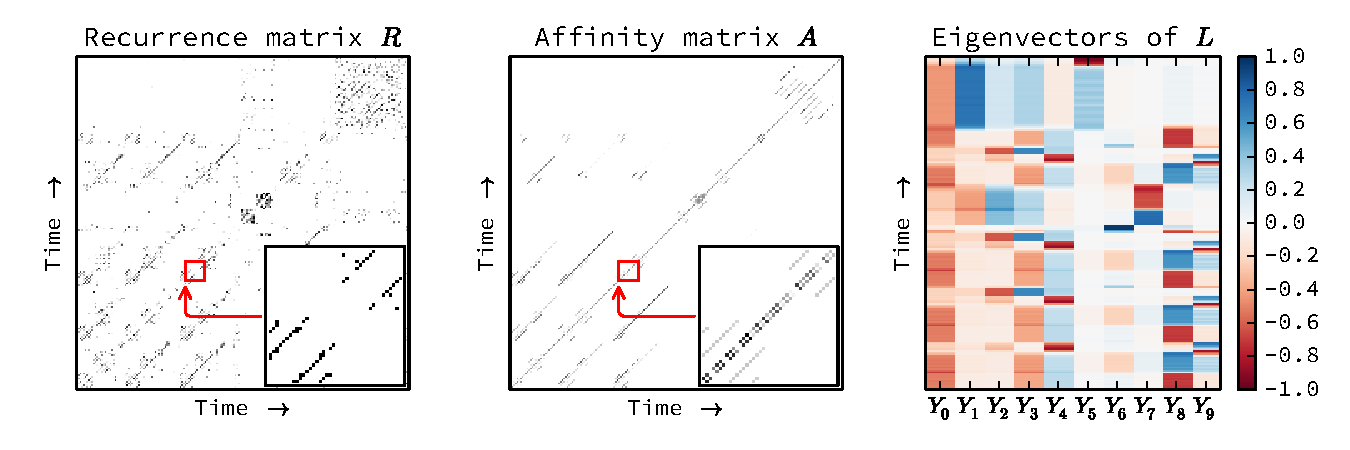
\includegraphics[width=\textwidth]{figs/recurrence}
\caption{Left: the recurrence matrix $R$ for \emph{The Beatles -- Come
Together}. Center: the sequence-augmented affinity matrix $A$.
Right: the first 10 basis features (columns), ordered left-to-right.  
The leading columns encode the primary structural components, while subsequent components represent structural refinements (individual measures).\label{recurrence}}
\end{figure*}

 
\begin{figure*}
\centering
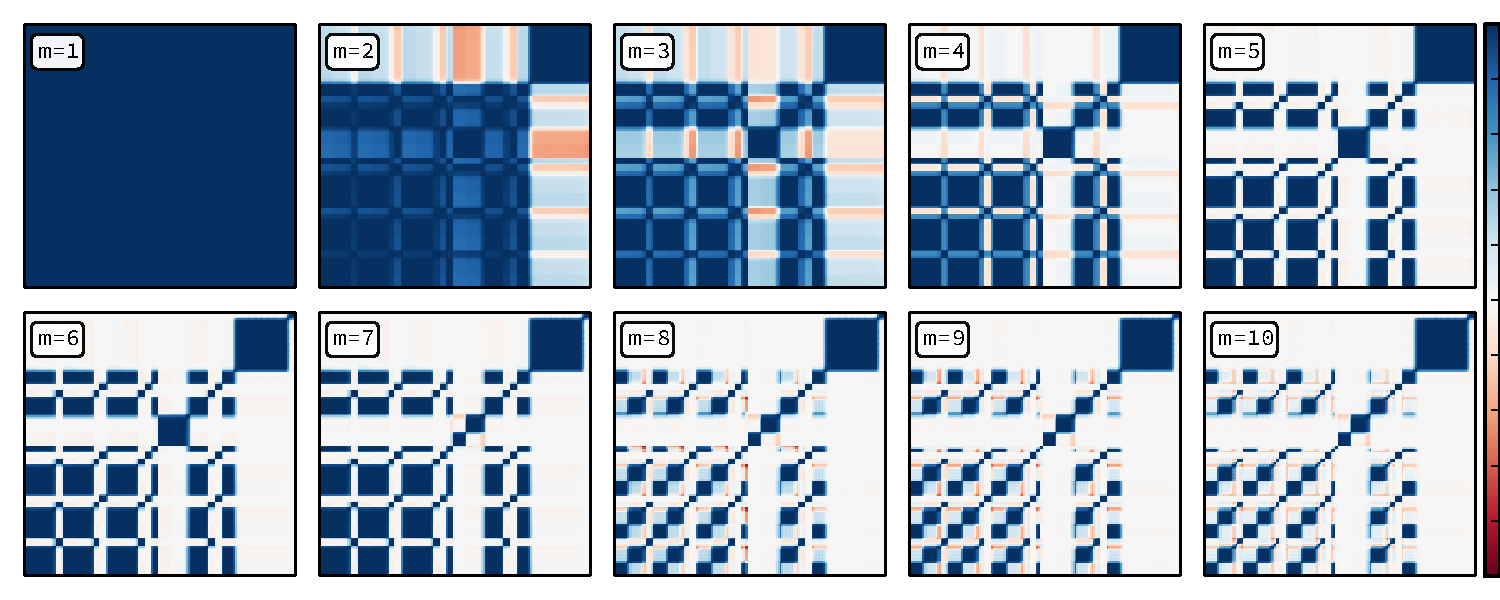
\includegraphics[width=\textwidth]{figs/lowrank}
\caption{Pairwise frame similarity using the first $10$ components for \emph{The Beatles -- Come Together}.  The first
(trivial) component ($m=1$) captures the entire song, and the second ($m=2$) separates
the outro from the rest of the song.  Subsequent refinements separate the solo,
refrain, verse, and outro, and then refine each component into individual measures.\label{lowrank}}
\end{figure*}

\section{Algorithms}

\subsection{Change-point detection}

\begin{algorithm}
\caption{Change-point detection\label{cpd}}
\begin{algorithmic}[1]
\REQUIRE{Repetition features $Y \in \R^{M \times n}$, $2 \leq k_\text{min}$}
\ENSURE{Boundaries $B^*$, number of segment labels $m^*$}\\
{\sc CPD}$(Y, k_\text{min}, k_\text{max})$
    \STATE{$B^* \leftarrow \emptyset$}
    \FOR{$m \leftarrow 1, 2, \ldots, M$}
        \STATE{Let $\hat{y}_t \leftarrow Y_{1:m, t} / \|Y_{1:m, t}\|^2$}\\
        \COMMENT{Truncate and normalize the columns of $Y$}
        \STATE{Run $k$-means on $\{\hat{y}_t\}_{i=1}^n$ with $k=m$}
        \STATE{Let $c_t$ be the cluster containing $\hat{y}_t$}
        \STATE{$B \leftarrow \{t \given c_t \neq c_{t+1}\}$}
        \IF{$B^* = \emptyset$ or $k_\text{min} \leq |B| + 1 \leq k_\text{max}$} 
        \STATE{$B^* \leftarrow B, \quad m^* \leftarrow m$}
        \ENDIF
    \ENDFOR
    \RETURN{$B^*, m^*$}
\end{algorithmic}
\end{algorithm}

\subsection{Structure annotation}

\begin{algorithm}
\caption{Laplacian structural decomposition\label{lss}}
\begin{algorithmic}[1]
\REQUIRE{ Affinities: $S^\text{rep}, S^\text{loc} \in \R_+^{n\times n}$\\
maximum number of segment types: $M$\\
bounds on the number of segments: $2 \leq k_\text{min} < k_\text{max}$}
\ENSURE{Segment boundaries $B$, labels $C$}\\
{\sc LSD}$(S^\text{rep}, S^\text{loc}, k_\text{min}, k_\text{max}$)
\STATE{$R' \leftarrow $ filtered recurrence matrix of $S^\text{rep}$ (\Cref{filtered-rep})}
\STATE{$A \leftarrow $ sequence-augmented affinity matrix (\Cref{saam})}
\STATE{$L \leftarrow I - D^{-1/2} A D^{-1/2}$}
\STATE{$Y \leftarrow$ bottom $M$ eigenvectors of $L$}
\STATE{$B \leftarrow \text{\sc CPD}(Y, k_\text{min}, k_\text{max})$
\COMMENT{\Cref{cpd}}}
\STATE{$S_i \leftarrow$ mean of $Y^{m}$ over $[B_i, B_{i+1})$}
\STATE{Run $k$-means on $S$ with $k=m$}
\STATE{Let $C_i$ be the cluster containing the $i$th segment}
\RETURN{$B, C$}
\end{algorithmic}
\end{algorithm}

% For each m in 2 .. M:
% m <- argmax gap
% compute segment centroids over boundaries[m], and cluster by k-means with k=m
% return boundary times and segment labels

\section{Experiments}

\subsection{Data}

\subsection{Implementation}

\subsection{Results}

\section{Discussion}

\bibliography{refs}

\end{document}
